\documentclass{article}
\usepackage{spconf,amsmath,graphicx}
\usepackage{booktabs}
\usepackage{xcolor}
\usepackage{hyperref}

% Red marker for numbers that await running experiments; must be empty before submission.
\newcommand{\pending}[1]{\textcolor{red}{[#1]}}

\title{Site-Probe Accuracy Is Not a Harmonization Score:\\
An Audit of Evaluation Practice for Multi-Site MRI}

\name{
\parbox{\textwidth}{\centering
Muhammad Muqsit Islam$^{1,2,\star,\dagger}$\thanks{$^\star$Corresponding author}\thanks{$^\dagger$ Equal contribution}
\qquad
Gloria García Cuenco$^{1,2,\dagger}$ \\
\qquad José M. Martínez Sánchez$^{1}$ \qquad
Pierrick Coupé$^{2}$ \qquad \\
}}

\address{$^{1}$ Universidad Autónoma de Madrid, Spain \\
$^{2}$ University of Bordeaux, France}

\begin{document}
\maketitle

\begin{abstract}
Image-level MRI harmonization is often scored by how poorly a frozen site classifier recognizes the acquisition site of harmonized images, together with similarity to the input. We audit this practice on raw ABIDE~I T1-weighted MRI (1,112 subjects, 17 sites), treating ten test outputs from seven method families harmonized toward one target site as test cases rather than contestants. Using subject-level paired bootstrap intervals, a valid shuffled-label control and target-site subjects reported separately, we find that: (i) the site accuracy assigned to a method depends on the probe checkpoint, and a probe retrained with the same recipe rated three methods as retaining 1.7 to 2.1 times as much site information; (ii) the lowest site accuracy, at chance, came from the most destructive output, which also moved intensities away from the target; (iii) a small change from the input did not imply alignment with the target: diffusion translation changed intensities least but moved them no closer to the target; and (iv) for all three methods tested, probes trained on the harmonized images recovered the source site almost as well as from raw images (balanced accuracy 0.87--0.91 versus 0.33--0.45 for probes trained on raw slices). Head silhouettes alone identified sites (0.73--0.86), and an intensity-histogram probe separated the cases: histogram matching removed intensity site information (0.16), whereas CycleGAN (0.74) and diffusion (0.70) retained it near the raw level (0.74). We release the evaluator and propose a reporting checklist.
\end{abstract}

\begin{keywords}
MRI harmonization, evaluation, site classification, domain shift, reproducibility
\end{keywords}

\section{Introduction}
\label{sec:intro}
Pooling MRI across sites introduces acquisition differences that confound downstream analyses and degrade models on unseen scanners~\cite{fortin2018harmonization,glocker2019multisite}. Image-level harmonization translates scans toward a common appearance, but paired scans of the same subject on every scanner are rarely available, so methods are judged indirectly~\cite{hu2023harmonization}. A common proxy is a \emph{site probe}: a classifier trained to recognize the acquisition site on unharmonized images and then applied, frozen, to harmonized ones~\cite{glocker2019multisite,dinsdale2021unlearning}. Lower probe accuracy is read as removal of site information and is typically paired with similarity to the input, such as PSNR, and with intensity-distribution distances.

Each proxy measures less than it appears to. A frozen probe reports what one classifier can still recover; it can also fail because the harmonized images are unfamiliar to it, damaged, or noisy. In representation learning, removing an attribute until a fixed adversary fails does not stop a newly trained classifier from recovering it~\cite{elazar2018adversarial}. Similarity to the input rewards doing nothing, and a small distribution distance between input and output says nothing about the target site. Without paired data these ambiguities cannot be resolved by one number, yet benchmark tables routinely rank methods on such numbers.

We audit these practices on outputs of seven harmonization families. Our contributions are: (1) a subject-level evaluation protocol with paired uncertainty, valid probe controls, separate reporting of target-site subjects, and target alignment measured apart from change; (2) evidence that probe verdicts depend on the probe checkpoint, that the lowest site accuracy can signal destruction, and that small change does not imply alignment; (3) a test of whether low accuracy reflects removed or hidden site information, using probes trained on harmonized images, with geometry-only and intensity-only controls; and (4) a reporting checklist. We do not propose a harmonizer, and we do not rank the audited methods.

\section{Data and Audited Outputs}
\label{sec:data}
\textbf{Cohort.} We use raw ABIDE~I T1-weighted scans~\cite{dimartino2014abide}: 1,112 subjects from 17 sites, split by subject and stratified by site into 890 training, 113 validation and 109 test subjects. Volumes are reoriented, clipped to foreground percentiles $[p_1,p_{99}]$ and scaled to $[0,1]$ with background at zero. One axial slice per subject is chosen by foreground area, cropped with a dilated head mask and resized to $256\times256$. NYU, the largest site, is the harmonization target; 19 test subjects are from NYU and 90 from the 16 source sites. For 4 of 109 test subjects two candidate slices tie exactly, and one tie was broken differently on another machine, so the chosen slices are frozen and verified for every output.

\textbf{Audited outputs.} Test outputs from earlier benchmark runs were evaluated without retraining or retuning: NeuroCombat~\cite{johnson2007combat,fortin2018harmonization} applied per pixel and fit on the test cohort itself (transductive); histogram matching of foreground quantiles to a pooled 17-site training reference~\cite{nyul2000standardization}; CycleGAN~\cite{zhu2017cyclegan}; StarGAN~\cite{choi2018stargan} with aggressive and conservative settings; DLEST~\cite{wu2025dlest} after 1,000 and 1,500 steps; conditional diffusion image-to-image translation~\cite{ho2020ddpm,meng2022sdedit} (strength 0.35, 50 DDIM steps); and adapted volumetric HCLD~\cite{wu2026hcld}, from which the frozen slice was extracted. Learned methods were trained on the training split. Generators return NYU inputs unchanged up to numerical precision, whereas NeuroCombat and histogram matching alter them. Because the test subjects were inspected during the earlier benchmark, this is a retrospective reanalysis; all audit experiments were fixed in a written protocol before their outcomes were seen, and later amendments record what had been observed.

\section{Audit Protocol}
\label{sec:protocol}
\textbf{Change and target alignment.} On whole images we compute PSNR on a fixed intensity scale ($[0,1]$) and normalized cross-correlation (XCorr) between input and output. Exact identities have infinite PSNR, so summaries are reported for the 90 source subjects, with NYU reported separately. We distinguish \emph{change}, the per-subject Wasserstein-1 distance between input and output intensities, from \emph{target alignment}: the Wasserstein-1 distance and KL divergence between an image's foreground intensities and a reference built from raw fixed slices of the 147 NYU training subjects, each weighted equally. Foreground is defined on the raw slice, never on a method's output, and $\Delta W_{\mathrm{NYU}}$ is the output's distance minus the input's.

\textbf{Site probes.} All probes are ResNet-18 networks~\cite{he2016resnet} with single-channel input, predicting 17 sites and trained with AdamW (learning rate $3\times10^{-4}$, batch 64, 500 steps) and random affine augmentation. The \emph{frozen} probe is the checkpoint used by the earlier benchmark. \emph{Retrained} probes use the same recipe with seeds 42 and 1--4 and random valid slices from the training volumes; each is selected on full validation balanced accuracy (BA) and evaluated once. A shuffled-label control permutes site labels between subjects within each split, keeping class counts and labels fixed across slices. To separate removed from hidden site information, \emph{slice probes} are trained, with the same recipe, on the fixed training and validation slices of either raw images or one method's outputs, for three methods chosen in advance to cover intensity, adversarial and diffusion families (seeds 1--3). Two controls, added after the first slice-probe results and before their own, restrict what a probe can see: slice probes on filled binary head silhouettes (geometry only), and multinomial logistic regression on 50-bin foreground intensity histograms (intensity only; regularization chosen on validation), trained on raw slices or on a method's outputs.

\textbf{Statistics.} Site BA on source subjects is macro-averaged over the 16 source sites (chance 1/16). Intervals are 95\% percentile intervals from 2,000 bootstrap replicates that resample subjects within each site, reusing the same replicates across methods and probes so that comparisons are paired. They describe uncertainty over subjects given fixed checkpoints; variation over probe training seeds is reported separately.

\begin{table*}[t]
\centering
\caption{Source-subject results ($n=90$). PSNR and XCorr compare output with input; $\Delta W_{\mathrm{NYU}}$ is the change in Wasserstein-1 distance to the NYU reference (negative is closer). Site BA: frozen probe with 95\% subject-bootstrap interval; retrained site probes as mean [min, max] over seeds; image slice probes (mean over seeds) and intensity-histogram probes, each trained on raw slices $\rightarrow$ on the method's own outputs. Raw-input BA is on unharmonized images; chance is 0.06. $^\dagger$Fit on the test cohort. $^\ddagger$Pooled 17-site reference.}
\label{tab:main}
\footnotesize
\setlength{\tabcolsep}{3.5pt}
\begin{tabular}{@{}lccccccc@{}}
\toprule
 & \multicolumn{3}{c}{Change and target alignment} & \multicolumn{4}{c}{Source-site balanced accuracy (probe trained on raw $\rightarrow$ on outputs)} \\
\cmidrule(lr){2-4}\cmidrule(l){5-8}
Method & PSNR & XCorr & $\Delta W_{\mathrm{NYU}}$ & Frozen & Retrained & Image probe & Intensity probe \\
\midrule
Raw input & -- & -- & 0 & 0.95 & 0.90 [0.81, 0.98] & 0.92 & 0.74 \\
NeuroCombat$^\dagger$ & 20.0 & 0.940 & +0.003 & 0.27 [0.21, 0.32] & 0.33 [0.26, 0.37] & 0.36 & 0.11 \\
Histogram matching$^\ddagger$ & 23.0 & 0.982 & -0.053 & 0.44 [0.37, 0.52] & 0.44 [0.27, 0.59] & 0.45 $\rightarrow$ 0.87 & 0.08 $\rightarrow$ 0.16 \\
CycleGAN & 21.3 & 0.977 & -0.036 & 0.31 [0.25, 0.37] & 0.28 [0.13, 0.59] & 0.33 $\rightarrow$ 0.87 & 0.21 $\rightarrow$ 0.74 \\
StarGAN (aggr.) & 16.0 & 0.896 & -0.019 & 0.21 [0.15, 0.27] & 0.35 [0.18, 0.54] & 0.39 & 0.21 \\
StarGAN (cons.) & 26.9 & 0.991 & -0.021 & 0.83 [0.79, 0.86] & 0.78 [0.66, 0.89] & 0.82 & 0.34 \\
DLEST 1500 & 26.6 & 0.993 & -0.020 & 0.67 [0.61, 0.72] & 0.73 [0.65, 0.82] & 0.76 & 0.42 \\
DLEST 1000 & 28.4 & 0.993 & -0.009 & 0.71 [0.65, 0.77] & 0.84 [0.76, 0.89] & 0.82 & 0.47 \\
Diffusion img2img & 21.7 & 0.948 & -0.001 & 0.37 [0.32, 0.42] & 0.42 [0.24, 0.63] & 0.44 & 0.36 \\
\quad second draw & 21.7 & 0.948 & -0.002 & 0.35 [0.29, 0.40] & 0.42 [0.30, 0.62] & 0.41 $\rightarrow$ 0.91 & 0.37 $\rightarrow$ 0.70 \\
Adapted HCLD & 13.9 & 0.706 & +0.108 & 0.07 [0.06, 0.08] & 0.08 [0.06, 0.11] & 0.07 & 0.07 \\
\bottomrule
\end{tabular}

\end{table*}

\begin{figure}[t]
\centering
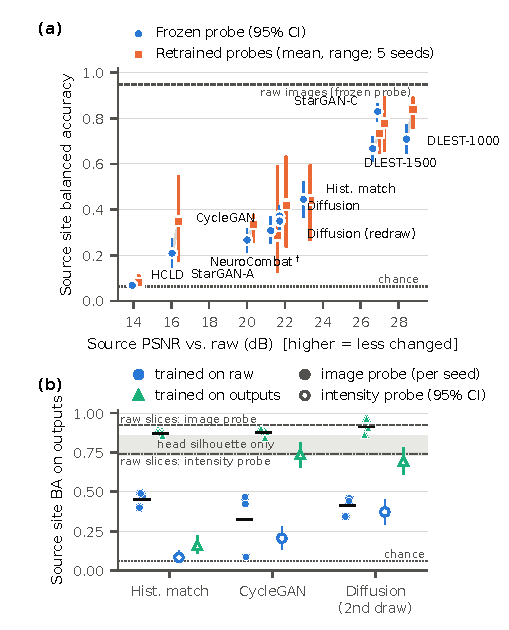
\includegraphics[width=\linewidth]{figures/fig_probe_verdicts.pdf}
\caption{(a) Site BA versus change from the input for each output. Blue: frozen probe with 95\% interval; orange: retrained probes (mean and range over seeds), joined to the frozen estimate. (b) Probes trained on raw slices (blue) or on each method's outputs (aqua), evaluated on that method's test outputs: image slice probes (filled, one per seed, bar at mean) and intensity-histogram probes (hollow, 95\% interval). Band: image probes given only head silhouettes.}
\label{fig:verdicts}
\end{figure}

\section{Results}
\label{sec:results}
\textbf{Probe validity.} On unharmonized source images the frozen probe reached BA 0.95 [0.90, 1.00] and the seed-42 retrained probe 0.81 [0.75, 0.87] \pending{seeds 1--4}. The shuffled-label control scored 0.03 [0.01, 0.05], at chance, so the probes learn site-related structure rather than label artifacts. That structure need not be scanner appearance: slice probes given only filled head silhouettes identified source sites with BA 0.77, 0.86 and 0.73 (seeds 1--3), and a logistic-regression probe given only foreground intensity histograms reached 0.74 [0.65, 0.84].

\textbf{Verdicts depend on the probe.} With the same recipe, the retrained probe changed the site BA assigned to several outputs by more than their interval widths (Table~\ref{tab:main}, Fig.~\ref{fig:verdicts}a): diffusion rose from 0.37 to 0.63, CycleGAN from 0.31 to 0.59 and aggressive StarGAN from 0.21 to 0.44, while NeuroCombat (0.27 vs.\ 0.26) and HCLD (0.07 vs.\ 0.09) were unchanged. For DLEST~1000 the retrained probe assigned a higher BA to harmonized outputs (0.85) than to raw images (0.81), which cannot mean that harmonization added site information; it indicates that each checkpoint responds differently to the distribution shift an output introduces. \pending{Across five seeds, site BA ranges and method-ranking agreement (Kendall $\tau$).}

\textbf{The lowest site accuracy came from destruction.} HCLD reached BA 0.07 [0.06, 0.08], at chance, under the frozen probe and 0.09 [0.06, 0.13] under the retrained one, with the lowest PSNR (13.9~dB) and XCorr (0.71) of any output, and it moved intensities away from the target ($\Delta W_{\mathrm{NYU}}=+0.108$). Aggressive StarGAN had the second-lowest frozen BA and the second-lowest PSNR. Averaging over all 109 subjects would add 19 NYU subjects that the generators return exactly or almost exactly unchanged (PSNR infinite or above 150~dB); such pooled summaries are undefined or dominated by target identities.

\textbf{Small change is not target alignment.} Diffusion translation changed intensities the least (input-to-output $W=0.008$), yet it moved them no closer to NYU ($\Delta W_{\mathrm{NYU}}=-0.0013$ [$-0.0023$, $-0.0004$]) and increased the KL divergence to NYU from 0.30 to 0.83. Histogram matching ($-0.053$) and CycleGAN ($-0.036$) moved intensities toward the target; NeuroCombat did not ($+0.003$ [$-0.001$, $0.008$]). Diffusion outputs are also a random draw: re-sampling the same checkpoint on the same inputs gave images that differed from the first draw by a mean foreground absolute difference of 0.085, more than their mean difference from the input (0.075), with unchanged mean PSNR (21.71 vs.\ 21.73~dB). Site BA changed little between draws (frozen 0.37 vs.\ 0.35; retrained 0.63 vs.\ 0.62), far less than between probes.

\textbf{Removed or hidden?} Slice probes trained on raw slices recognized sites on raw test slices with BA 0.92 (range over seeds 0.88--0.97); their shuffled-label control scored 0.07 [0.03, 0.10]. Applied to harmonized outputs, these probes gave 0.45 for histogram matching, 0.33 for CycleGAN (0.09--0.47 across seeds) and 0.41 for diffusion, the kind of drop usually reported as harmonization. Probes trained on each method's own outputs, however, recovered the source site from that method's test outputs with BA 0.87 (0.85--0.88), 0.87 (0.84--0.90) and 0.91 (0.86--0.97), close to the raw ceiling (Fig.~\ref{fig:verdicts}b, Table~\ref{tab:main}); for every seed the two probes' intervals were disjoint, and final-epoch checkpoints led to the same conclusion. Because head geometry alone identifies sites, this shows that site remains recoverable, not which channel carries it. The intensity-only probe separates the methods. Trained on raw slices it dropped to 0.08, 0.21 and 0.37 on the three outputs, mirroring the image probes. Trained on the outputs, it recovered little from histogram matching (0.16 [0.11, 0.22]), whose intensity distributions are matched by construction, but recovered CycleGAN (0.74 [0.65, 0.81]) and diffusion (0.70 [0.61, 0.78]) outputs about as well as raw slices (0.74). CycleGAN and diffusion therefore transformed rather than removed the site-specific intensity signature, and probes trained on diffusion outputs even recognized sites on raw test images (0.78--0.93).

\section{Discussion and Recommendations}
\label{sec:discussion}
No single probe number identifies a good harmonizer. Low site accuracy from a frozen probe arose from probe-specific sensitivity, from destruction of the image, and, for every method we could test, from site information that a probe trained on harmonized images readily recovered; a small change from the input was compatible with no movement toward the target. Site labels are also a confounded target: they are predictable from head geometry, which intensity harmonization should preserve, so site accuracy of image probes cannot by itself certify scanner-effect removal. We therefore recommend that evaluations: (1) report site accuracy from several independently trained probes, including probes trained on harmonized outputs, and probes restricted to the channel the method is meant to change, rather than one frozen checkpoint; (2) report each probe's accuracy on raw images and a subject-level shuffled-label control; (3) measure alignment to a held-out target reference separately from change from the input; (4) exclude target-site identities from source summaries; (5) compute uncertainty over subjects, paired across methods, not over pixels or slices; (6) evaluate several sampling draws of stochastic generators; and (7) read low site accuracy together with fidelity, since low accuracy with low fidelity indicates destruction.

\textbf{Limitations.} The audit uses one cohort, one target site and one axial slice per subject, so through-plane and volumetric effects are not assessed. No anatomical ground truth is available: PSNR and XCorr measure agreement with the input, not correctness. Site labels are confounded with head geometry and with cohort demographics; our controls bound the geometric and intensity-histogram channels but do not isolate scanner effects from biological differences between sites. Generators were not retuned, and one baseline is transductive. The test subjects had been inspected previously, which motivated frozen protocols and documented amendments.

\section{Compliance with Ethical Standards}
\label{sec:ethics}
This research study was conducted retrospectively using human subject data made available in open access by ABIDE~I~\cite{dimartino2014abide}. Ethical approval was not required as confirmed by the license attached with the open access data.

\section{Acknowledgments}
\label{sec:acknowledgments}
\pending{Funding.} The authors have no relevant financial or non-financial interests to disclose. \pending{AI-use disclosure: wording to be approved by the authors.}

\bibliographystyle{IEEEbib}
\bibliography{refs}

\end{document}
